\documentclass[17pt]{beamer} %Makes presentation
%\documentclass[handout, 17pt]{beamer} %Makes Handouts
\documentclass[17pt]{beamer} %Makes presentation
%\documentclass[handout]{beamer} %Makes Handouts
\usetheme{Singapore} %Gray with fade at top
\useoutertheme[subsection=false]{miniframes} %Supppress subsection in header
\useinnertheme{rectangles} %Itemize/Enumerate boxes
\usecolortheme{seagull} %Color theme
\usecolortheme{rose} %Inner color theme

\definecolor{light-gray}{gray}{0.75}
\definecolor{dark-gray}{gray}{0.55}
\setbeamercolor{item}{fg=light-gray}
\setbeamercolor{enumerate item}{fg=dark-gray}

\setbeamertemplate{navigation symbols}{}
%\setbeamertemplate{mini frames}[default]
%\setbeamercovered{dynamics}
\setbeamerfont*{title}{size=\Large,series=\bfseries}
\setbeamerfont{footnote}{size=\tiny}

%\setbeameroption{notes on second screen} %Dual-Screen Notes
%\setbeameroption{show only notes} %Notes Output

\setbeamertemplate{frametitle}{\vspace{.5em}\bfseries\insertframetitle}
\newcommand{\heading}[1]{\noindent \textbf{#1}\\ \vspace{1em}}

\usepackage{bbding,color,multirow,times,ccaption,tabularx,graphicx,verbatim,booktabs}
\usepackage{colortbl} %Table overlays
\usepackage[english]{babel}
%\usepackage[latin1]{inputenc}
%\usepackage[T1]{fontenc}
\usepackage{lmodern}

%\author[]{Thomas J. Leeper}
\institute[]{
  \inst{}%
  Department of Government\\London School of Economics and Political Science
}


\title{Description and Evidence Gathering}



\date[]{}

\begin{document}

\frame{\titlepage}

\frame{\tableofcontents}

\section{Review}
\frame{\tableofcontents[currentsection]}

\frame{

\frametitle{Preview}

\small

\begin{itemize}\itemsep0.5em
\item You have everything you need to complete:
	\begin{itemize}
	\item Problem set 2 (Concepts)
	\item Problem set 3 (Measurement)
	\end{itemize}
\item<2-> Next week is reading week (no lecture or class)
\item<3-> Week 7 -- Online lecture + guest lecture
\item<4-> Start thinking about what kinds of topics interest you as possible research proposals
\end{itemize}

}


\frame{

\frametitle{Review}

\begin{itemize}\itemsep0.5em
\item Data Description
\item Variable summaries
	\begin{itemize}
	\item Statistics
	\item Tabulation
	\item Aggregation
	\end{itemize}
\item Visualisation
\end{itemize}

}


\frame{
\frametitle{Anscombe's Quartet}

\begin{center}
{\tiny
\begin{tabular}{rr rr rr rr}
\multicolumn{2}{c}{I} & 
\multicolumn{2}{c}{II} & 
\multicolumn{2}{c}{III} & 
\multicolumn{2}{c}{IV}\\
10.0&8.04&10.0&9.14&10.0&7.46&8.0&6.58\\
8.0&6.95&8.0&8.14&8.0&6.77&8.0&5.76\\
13.0&7.58&13.0&8.74&13.0&12.74&8.0&7.71\\
9.0&8.81&9.0&8.77&9.0&7.11&8.0&8.84\\
11.0&8.33&11.0&9.26&11.0&7.81&8.0&8.47\\
14.0&9.96&14.0&8.10&14.0&8.84&8.0&7.04\\
6.0&7.24&6.0&6.13&6.0&6.08&8.0&5.25\\
4.0&4.26&4.0&3.10&4.0&5.39&19.0&12.50\\
12.0&10.84&12.0&9.13&12.0&8.15&8.0&5.56\\
7.0&4.82&7.0&7.26&7.0&6.42&8.0&7.91\\
5.0&5.68&5.0&4.74&5.0&5.73&8.0&6.89\\
\end{tabular}
}
\end{center}

\vspace{0.5em}

$\bar{x}=9$, $Var(x)=11$,\\
$\bar{y} = 7.5$, $Var(y)=4.12$,\\
$Corr(x,y) = 0.816$
}

\frame{
\frametitle{Anscombe's Quartet}
\begin{center}
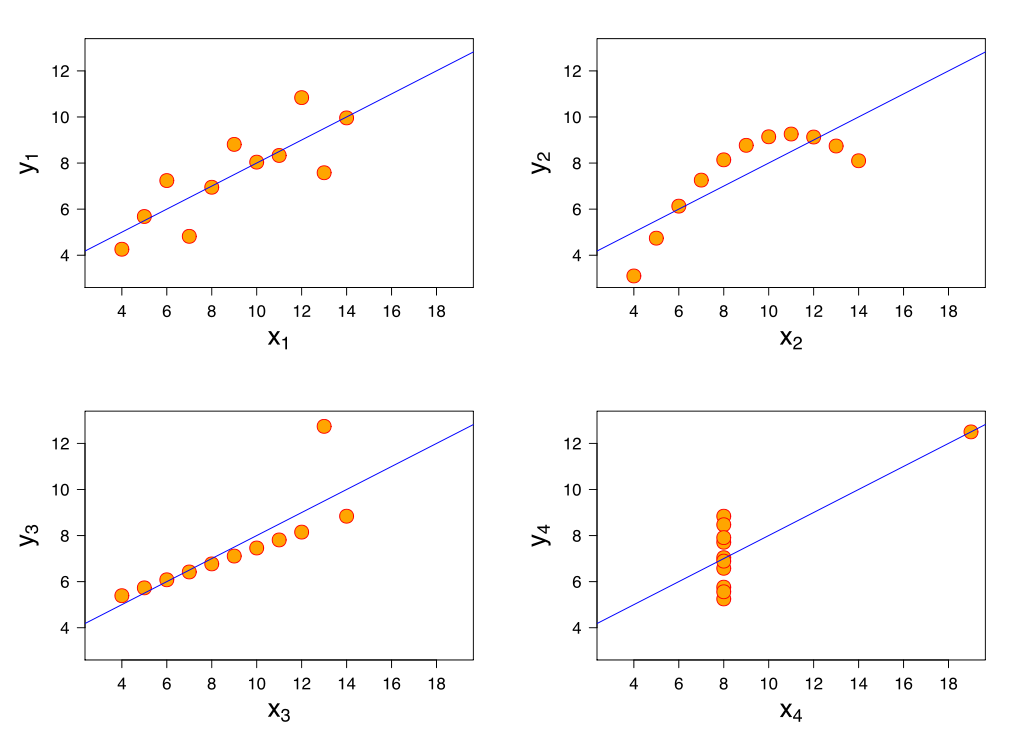
\includegraphics[height=.7\textheight]{images/anscombe.png}
\end{center}
\vspace{0.5em}
{\tiny Source: \href{https://commons.wikimedia.org/wiki/File:Anscombe\%27s_quartet_3.svg}{Wikimedia}}
}


\frame{
\frametitle{{\normalsize Simpson's Paradox}}
\begin{center}
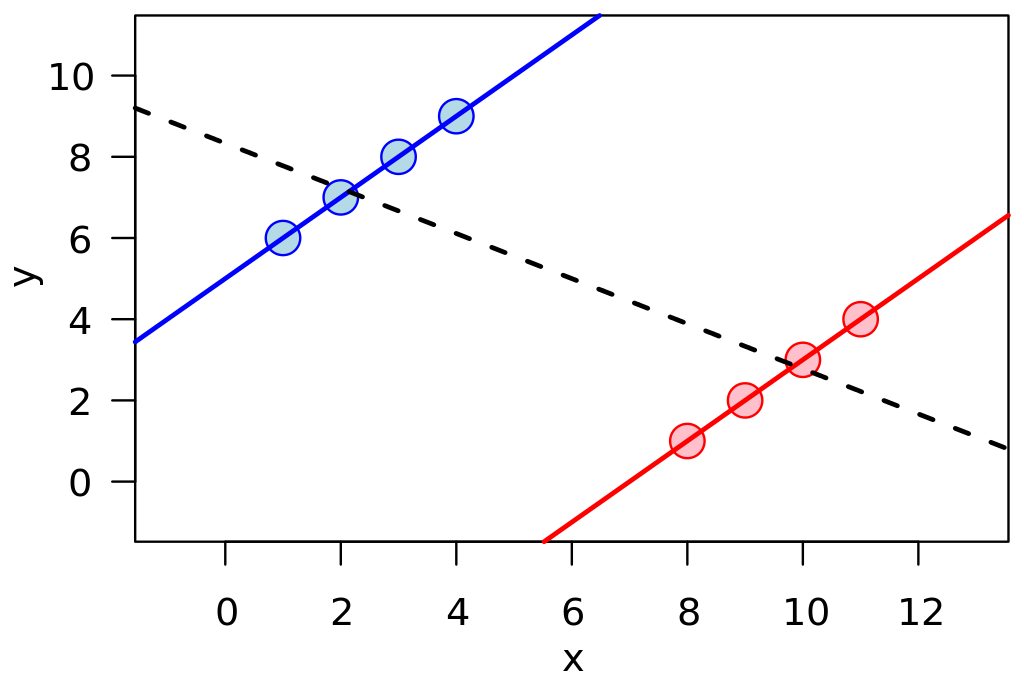
\includegraphics[height=.65\textheight]{images/simpsons.png}
\end{center}
\vspace{0.5em}
{\tiny Source: \href{https://commons.wikimedia.org/wiki/File:Simpson\%27s_paradox_continuous.svg}{Wikimedia}}
}


\frame{
%\frametitle{{\normalsize William Playfair}}
\begin{center}
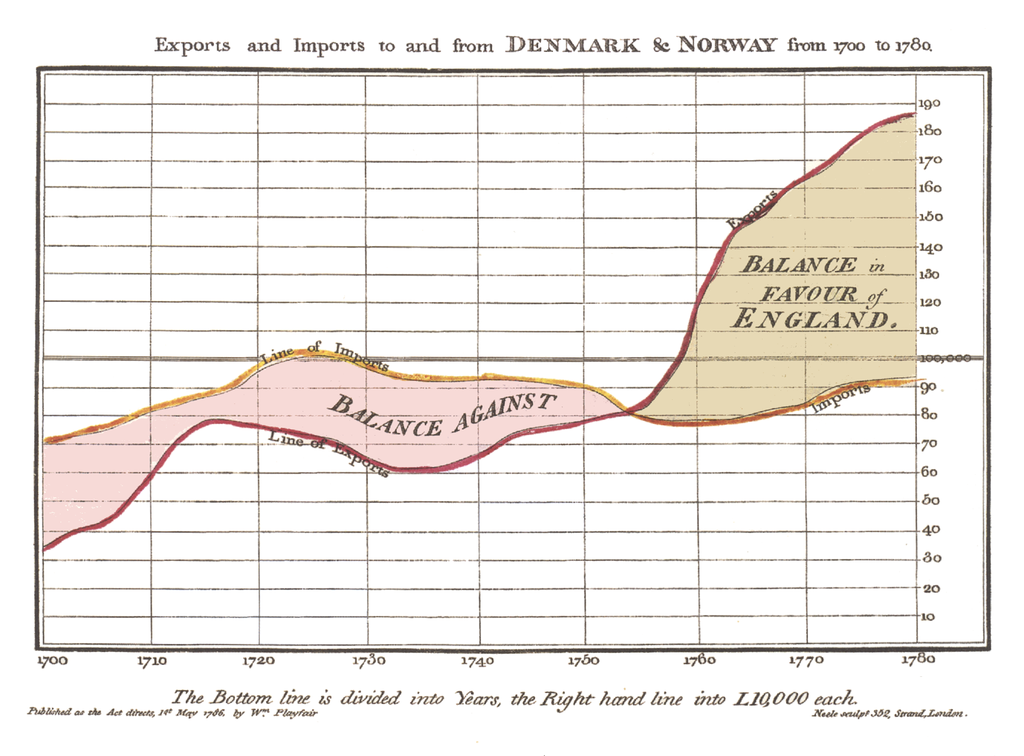
\includegraphics[width=\textwidth]{images/playfair.png}
\end{center}
{\tiny Source: \href{https://commons.wikimedia.org/wiki/File:Minard.png}{Wikimedia}}
}


\frame{
%\frametitle{{\normalsize Charles Minard}}
\begin{center}
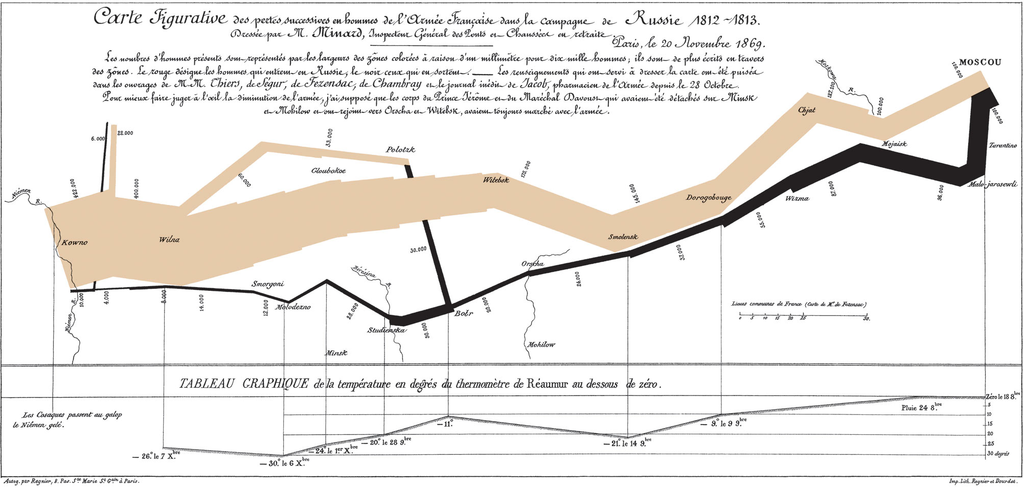
\includegraphics[width=1.05\textwidth]{images/minard.png}
\end{center}
{\tiny Source: \href{https://commons.wikimedia.org/wiki/File:Playfair_TimeSeries-2.png}{Wikimedia}}
}

\frame{
%\frametitle{{\normalsize Florence Nightingale}}
\begin{center}
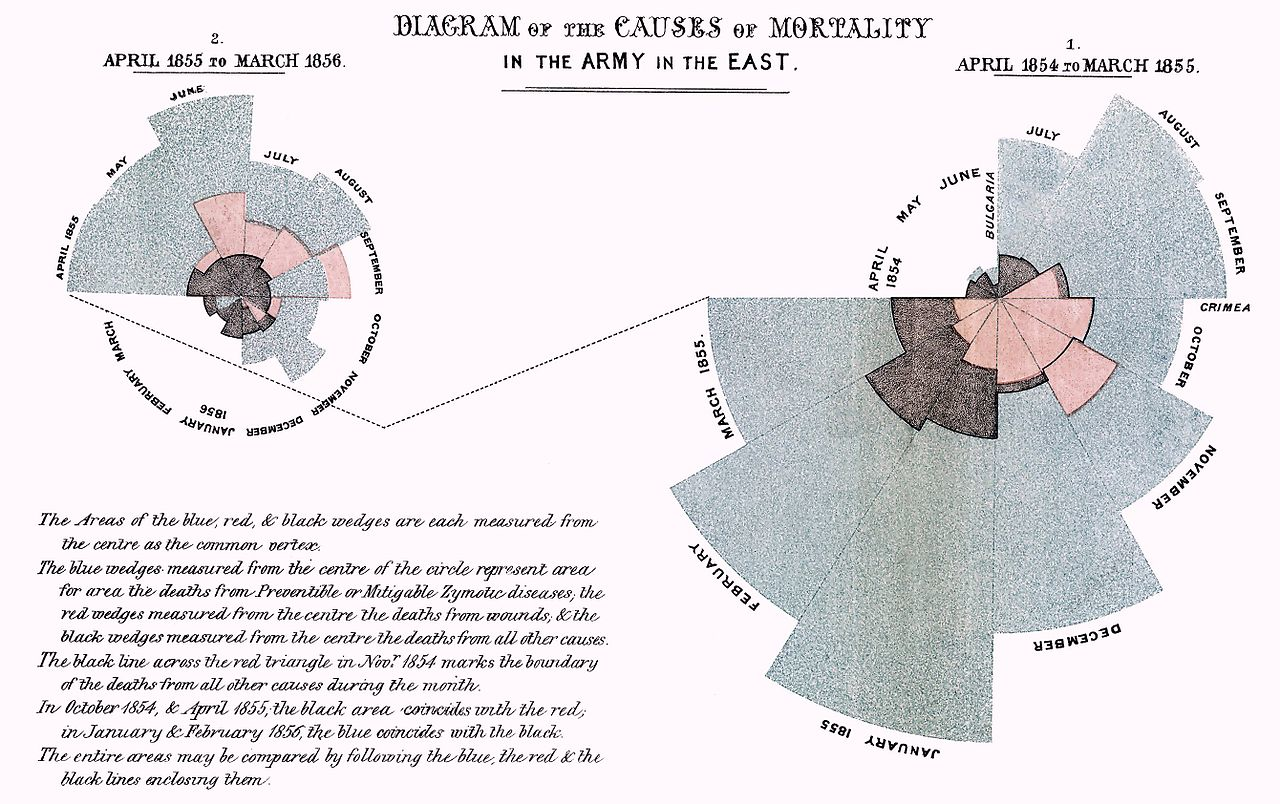
\includegraphics[height=.7\textheight]{images/rose.png}
\end{center}
\vspace{-0.5em}
{\tiny Source: \href{https://commons.wikimedia.org/wiki/File:Nightingale-mortality.jpg}{Wikimedia}}
}


\frame{
\frametitle{The bottom line}

A visualization should be a display of quantitative (and/or qualitative) data that tells an information-rich story in an honest and beautiful manner.
}




\frame{}


\section{Description}
\frame{\tableofcontents[currentsection]}



\frame{

\frametitle{{\large ``Description''}}

\small 

\begin{itemize}\itemsep0.25em
\item ``Description'' is a label for many practices
	\begin{itemize}
	\item Meaning is ambiguous
	\end{itemize}
\item<2-> Gerring describes many forms of description
	\begin{itemize}
	\item Summaries, associations
	\item Grouping/categorization (e.g., typologies)
	\item Accounts (e.g., biography, history)
	\end{itemize}
\item<3-> Toshkov has a different typology
	\begin{itemize}
	\item Multi-/single-case
	\item Multi-/uni-variate
	\end{itemize}
\end{itemize}

}

\frame{

\frametitle{Description $\equiv$ ``What?''}

A common feature of descriptive research and descriptive research questions is a focus on \textit{what} questions.

}


\frame[label=what]{

\frametitle{ ``What?'' Questions}
\begin{itemize}
\item<2-> What is this?
\item<3-> What other things are (un)like this?
\item<4-> What features does this have?
\item<5-> What people, institutions, and ideas does this involve?
\item<6-> Where is this? When is this? What happened before and after?
\item<7-> How much of this is there?
\end{itemize}

}

\frame{

\frametitle{Answering Descriptive RQs}

\begin{enumerate}\itemsep0.5em
\item Ask question
\item Decide what kind of evidence will answer that question
\item Gather evidence
\item Analyse evidence
\item Draw inferences and make claims
\item (Iterate)
\end{enumerate}

}

\frame{

\frametitle{Ex.: Broad Street Cholera}

\begin{enumerate}\itemsep0.25em
\item<2-> Who is getting cholera?
\item<3-> DSOs about who is sick (\& not sick)
\item<4-> Interview patients or use medical records
\item<5-> Examine associations between cholera and patient characteristics
\item<6-> Inference: Geographical clustering
\item<7-> Iterate: What is different about this geographical area?
\end{enumerate}

}


\frame{}

\againframe<7>{what}

% the answers to many of these questions are not DSOs


\frame{

\frametitle{Description and DSOs}

Description might\dots

\begin{itemize}\itemsep1em
\item \dots explore a single case to generate one or more DSOs

\item \dots compare multiple DSOs or summaries thereof

\item \dots not involve DSOs at all

\end{itemize}

}


\begin{frame}[fragile]
\frametitle{Generating DSOs}
\footnotesize
\begin{verbatim}
            country continent lifeExp      pop
            Austria    Europe     79   8199783
  Equatorial Guinea    Africa      ?         ?
            Iceland    Europe     81    301931
               Iran      Asia     70  69453570
             Kuwait      Asia     77   2505559
            Lesotho    Africa     42   2012649
             Serbia    Europe     74  10150265
              Sudan    Africa     58  42292929
             Sweden    Europe     80   9031088
Trinidad and Tobago  Americas     69   1056608
\end{verbatim}
\end{frame}

% assigning values
% developing measures


\begin{frame}[fragile]
\frametitle{Comparing DSOs}
\footnotesize
\begin{verbatim}
            country continent lifeExp      pop
            Lesotho    Africa     42   2012649
  Equatorial Guinea    Africa     51    551201
              Sudan    Africa     58  42292929
\end{verbatim}
\end{frame}

% as simple as visualization
% as complex as in-depth case comparisons of
% invitation to start generating causal hypotheses


\begin{frame}
\frametitle{Beyond DSOs}

\begin{itemize}\itemsep1em
\item<2-> Sequencing
\item<3-> Characterisation of processes
\item<4-> Policy, content, or discourse analysis
\item<5-> Conceptualisation
\item<6-> Causal hypothesis generation
\end{itemize}

\end{frame}

\frame{}


\frame{

\frametitle{{\large Common Methods of Descriptive Evidence Gathering}}

\begin{itemize}\itemsep0.25em
\item Documentary analysis
	\begin{itemize}
	\item Archival research
	\item Text analysis
	\end{itemize}
\item Interviewing
	\begin{itemize}
	\item Surveys
	\item Elite interviews
	\item Focus groups
	\end{itemize}
\item Direct observation
	\begin{itemize}
	\item Participant--observation
	\end{itemize}
\end{itemize}

}


\frame{

\frametitle{Question $\rightarrow$ Method}

\Large\centering
The choice of what methods to use should \textbf{always} follow from the research question being asked.

}


\frame{

\frametitle{{\large Some RQ/Method Pairings}}

{\small
\begin{tabular}{p{2.5in}p{1.5in}}
\textbf{Research Question} & \textbf{Evidence} \\ \midrule
How do cases differ? & DSOs \\ \midrule
What do people think? & Interviewing \\ \midrule
What happened? & Archival analysis \\ \midrule
How does this institution work? & ?? \\ \midrule
\end{tabular}
}

\only<2->{Yet, we often use non-obvious methods, and multiple methods.}
}


\frame{

\frametitle{Considerations}

\begin{itemize}
\item<2-> How do we decide what kind of evidence is appropriate?
\item<3-> How do we arbitrate between conflicting evidence?
\item<4-> How do we decide if evidence is ``true''?
\item<5-> How do we know when we have ``enough'' evidence?
\end{itemize}

}



\section{Texts as Sources}
\frame{\tableofcontents[currentsection]}


\frame{

\frametitle{What counts as text?}

\begin{itemize}\itemsep1em
\item Primary sources
	\begin{itemize}
	\item Raw, original evidence
	\end{itemize}
\item Secondary sources
	\begin{itemize}
	\item Interpretations of raw evidence
	\end{itemize}
\item Tertiary sources
	\begin{itemize}
	\item Compendia or indices of two other types of sources
	\end{itemize}
\end{itemize}

}
% brainstorm examples


\frame{

\frametitle{How do you use texts?}

\small

\begin{itemize}\itemsep0.75em
\item Think about your own experience reading, interpreting, and interacting with textual sources for academic purposes (e.g, for writing a term paper).
\item With the person sitting next to you, discuss:
	\begin{enumerate}
	\item The process by which you try to understand the meaning and content of texts
	\item How you choose texts to read
	\end{enumerate}
\end{itemize}

}

\frame{

\frametitle{Use of Texts}

\begin{itemize}\itemsep1em
\item<1-> Text as description
	\begin{itemize}
	\item Rely on text in lieu of direct observation
	\item What do we gain? What do we lose?
	\end{itemize}
\item<2-> Text as DSOs
	\begin{itemize}
	\item Treat texts as units (see MT Week 7)
	\end{itemize}
\end{itemize}


}

% texts in lieu of observation
% we cannot see everything ourselves, so we rely on evidence

\frame{

\frametitle{Challenges of Text}

\begin{enumerate}\itemsep1em
\item Source ``Quality''
\item Subjectivity and differing perspectives
\item Historiography
\item Selection and confirmation bias
\end{enumerate}

\onslide<2->{But these are really the challenges of \textit{any} research!}

}


% define historiography

% texts are subjective

% selection bias -> when do we stop looking for evidence?
% -> how do we know that we have all of the evidence?
% -> If we go looking for information about a case as something, do we miss evidence that sees that case as a case of something else?






\appendix
\frame{}

\end{document}
